\documentclass[11pt]{article} 



\makeatletter
\renewcommand\section{\@startsection{section}{1}{\z@}%
                                  {-3.5ex \@plus -1ex \@minus -.2ex}%
                                  {2.3ex \@plus.2ex}%
                                  {\normalfont\large\bfseries}}
\makeatother

\addtolength{\oddsidemargin}{-.875in}
\addtolength{\evensidemargin}{-.875in}
\addtolength{\textwidth}{1.75in}
\addtolength{\topmargin}{-.875in}
\addtolength{\textheight}{1.75in}


\usepackage{amssymb}
\usepackage{amsmath}
\usepackage{amsthm}
\usepackage{graphicx,caption,subcaption}


\usepackage{titling}
\setlength{\droptitle}{-6em}
\posttitle{\par\end{center}\vspace{-4.8em}}

\newcommand{\R}{{\ensuremath{\mathbb{R}}} }
\newcommand{\Q}{{\ensuremath{\mathbb{Q}}} }
\newcommand{\C}{{\ensuremath{\mathbb{C}}} }
\newcommand{\N}{{\ensuremath{\mathbb{N}}} }
\newcommand{\Z}{{\ensuremath{\mathbb{Z}}} }

\newcommand{\sexion}{\addtocounter{section}{1} }


\newcommand{\hint}[1]{{(\emph{Hint:} #1)}} %This line shows hints
%\newcommand{\hint}[1]{} %Use this line to hide all hints


\usepackage{fancyhdr}
\pagestyle{fancyplain}
\renewcommand{\headrulewidth}{0pt}

\begin{document}

%\lhead{}
\rhead{Harmonic Motion}
\section{Problem}
A 5 kg object is suspended in a jar by a spring which exerts 5 N force when extende 2.5 m past its equilibrium. The jar is filled with a liquid chosen so as to critically damp the system. The object is displaced 1m from equilibrium, and released. Find $t_0$ so that $|x(t)| < .01 $ for all $t > t_0$.

\section{Solution}
Recall the relevant differential equation:
\[m x'' + \mu x' + kx  = f(t)\]
There is no forcing term. We are given $m= 5$. Compute $k$ with Hooke's Law
\[ F = -k x \Rightarrow 5 = k \cdot 2.5 \Rightarrow k = 2.\]
Since the system is critically damped we have
\[0 = \Delta = \mu^2 - 4 m k   \Rightarrow \mu = \sqrt{4 \cdot 5 \cdot 2} = 2 \sqrt{10}  \]

So our differential equation is just
\[5 x'' + 2 \sqrt{10} x' + 2 x =0\]
Solve the corresponding characteristic equation with the quadratic formula to get
\[ \lambda = \frac{- 2 \sqrt{10}}{2 \cdot 5} = - \frac{\sqrt{10}}{5}\]
with multiplicity two. The solution is therefore
\[x(t) = A e^{- \sqrt{10} t/ 5} + B t e^{- \sqrt{10} t/ 5}\]
with derivative
\begin{align*}x'(t) &= -A \frac{\sqrt{10}}{5} e^{- \sqrt{10} t/ 5} + B\left(e^{- \sqrt{10} t/ 5}   -t \frac{\sqrt{10}}{5} e^{- \sqrt{10} t/ 5}\right) \\ &= -A \frac{\sqrt{10}}{5} e^{- \sqrt{10} t/ 5} + Be^{- \sqrt{10} t/ 5} \left(1  -t \frac{\sqrt{10}}{5} \right) \end{align*}

We have initial conditions $x(0) = 1/2, x'(0) = 0$, so
\[x(0) = 1/2  = A\]
\[x'(0) = 0 = -A \frac{\sqrt{10}}{5}  + B  =  - \frac{1}{2} \frac{\sqrt{10}}{5} + B \Rightarrow B  = \frac{\sqrt{10}}{10} \]
and the final solution is
\[x(t) = \frac{1}{2} e^{- \sqrt{10} t/ 5} + \frac{\sqrt{10}}{10} t e^{- \sqrt{10} t/ 5} = \frac{1}{10}e^{- \sqrt{10} t/ 5} \left (5  + \sqrt{10} t \right) \]

\section{Analysis}
\[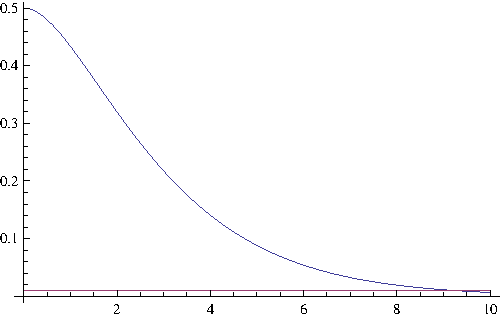
\includegraphics[scale =.9]{plot1}  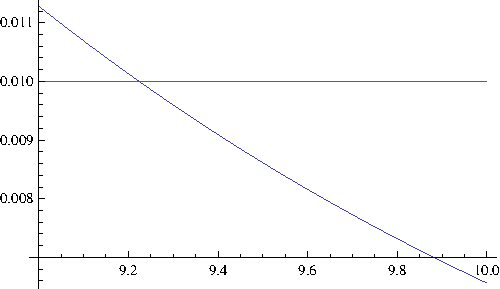
\includegraphics[scale =.9]{plot2}\]
Any candidate for $t_0$ must have $|x(t)| = .01$. So, since $x(t) > 0$ for $t> 0$  we solve
\[ \frac{1}{10}e^{- \sqrt{10} t/ 5} \left (5  + \sqrt{10} t \right) = .01\]
finding $t = -1.56942$, or $t = 9.22424$. We can discard the negative solution, so the only candidate is 
\[t_0 = 9.22424\]
To prove that we have $|x(t) |< .01$ for $t > t_0$ it suffices to note that $x(t) > 0$ for $t>0$, and 
\[x'(t) = -\frac{1}{2} \frac{\sqrt{10}}{5} e^{- \sqrt{10} t/ 5} + \frac{\sqrt{10}}{10}e^{- \sqrt{10} t/ 5} \left(1  -t \frac{\sqrt{10}}{5} \right) < 0 \mbox{ for } t >  9.22424\]


\end{document}
